% Copyright 2004 by Till Tantau <tantau@users.sourceforge.net>.
%
% In principle, this file can be redistributed and/or modified under
% the terms of the GNU Public License, version 2.
%
% However, this file is supposed to be a template to be modified
% for your own needs. For this reason, if you use this file as a
% template and not specifically distribute it as part of a another
% package/program, I grant the extra permission to freely copy and
% modify this file as you see fit and even to delete this copyright
% notice. 

\documentclass{beamer}

% There are many different themes available for Beamer. A comprehensive
% list with examples is given here:
% http://deic.uab.es/~iblanes/beamer_gallery/index_by_theme.html
% You can uncomment the themes below if you would like to use a different
% one:
%\usetheme{AnnArbor}
%\usetheme{Antibes}
%\usetheme{Bergen}
%\usetheme{Berkeley}
%\usetheme{Berlin}
%\usetheme{Boadilla}
%\usetheme{boxes}
%\usetheme{CambridgeUS}
%\usetheme{Copenhagen}
%\usetheme{Darmstadt}
%\usetheme{default}
%\usetheme{Frankfurt}
%\usetheme{Goettingen}
%\usetheme{Hannover}
%\usetheme{Ilmenau}
%\usetheme{JuanLesPins}
%\usetheme{Luebeck}
\usetheme{Madrid}
%\usetheme{Malmoe}
%\usetheme{Marburg}
%\usetheme{Montpellier}
%\usetheme{PaloAlto}
%\usetheme{Pittsburgh}
%\usetheme{Rochester}
%\usetheme{Singapore}
%\usetheme{Szeged}
%\usetheme{Warsaw}

\title{Words in Biology}
\setbeamertemplate{footline}
{
  \leavevmode%
  \hbox{%
  \begin{beamercolorbox}[wd=.333333\paperwidth,ht=2.25ex,dp=1ex,center]{author in head/foot}%
    \usebeamerfont{author in head/foot}\insertshortauthor%~~\beamer@ifempty{\insertshortinstitute}{}{(\insertshortinstitute)}
  \end{beamercolorbox}%
  \begin{beamercolorbox}[wd=.333333\paperwidth,ht=2.25ex,dp=1ex,center]{title in head/foot}%
    \usebeamerfont{title in head/foot}\insertshorttitle
  \end{beamercolorbox}%
  \begin{beamercolorbox}[wd=.333333\paperwidth,ht=2.25ex,dp=1ex,right]{date in head/foot}%
    \usebeamerfont{date in head/foot}\insertshortdate{}\hspace*{2em}
    \insertframenumber{} / \inserttotalframenumber\hspace*{2ex} 
  \end{beamercolorbox}}%
  \vskip0pt%
}
\setbeamertemplate{bibliography item}[text]
% A subtitle is optional and this may be deleted
%\subtitle{}

\author[Rahul and Srinidhi]{Rahul Kejriwal, CS14B023 \and Srinidhi Prabhu, CS14B028}
% - Give the names in the same order as the appear in the paper.
% - Use the \inst{?} command only if the authors have different
%   affiliation.

\date{}
\institute% (optional, but mostly needed)
{
  Indian Institute of Technology, Madras}
% - Use the \inst command only if there are several affiliations.
% - Keep it simple, no one is interested in your street address.

%\date{Conference Name, 2013}
% - Either use conference name or its abbreviation.
% - Not really informative to the audience, more for people (including
%   yourself) who are reading the slides online

%subject{Theoretical Computer Science}
% This is only inserted into the PDF information catalog. Can be left
% out. 

% If you have a file called "university-logo-filename.xxx", where xxx
% is a graphic format that can be processed by latex or pdflatex,
% resp., then you can add a logo as follows:

% \pgfdeclareimage[height=0.5cm]{university-logo}{university-logo-filename}
% \logo{\pgfuseimage{university-logo}}

% Delete this, if you do not want the table of contents to pop up at
% the beginning of each subsection:
%\AtBeginSubsection[]
%{
%  \begin{frame}<beamer>{Outline}
%    \tableofcontents[currentsection,currentsubsection]
%  \end{frame}
%}

% Let's get started
\begin{document}

\begin{frame}
  \titlepage
\end{frame}

\begin{frame}{Outline}
  \tableofcontents
  % You might wish to add the option [pausesections]
\end{frame}

% Section and subsections will appear in the presentation overview
% and table of contents.
\section{Motivation}

\begin{frame}{Motivation}{}
  \begin{itemize}
  	\item Proteins are strings composed of amino acids.
  	\item Subsequences of amino acids can be thought of as functional units in proteins.
  	\item Functional units in proteins can be seen as words of an unknown language.\footnote{\cite{tendulkar2013parallels}} \pause
  	\item Can we use existing methods to identify the words in the language of proteins?
  \end{itemize}
\end{frame}

\section{Approach}

% You can reveal the parts of a slide one at a time
% with the \pause command:
\begin{frame}{Approach}
  \begin{itemize}
  	\item To identify words from natural language texts, we use word segmentation algorithms.
  	\item Word segmentation algorithms can be of two types:
  	\begin{enumerate}
  		\item \textbf{Supervised:} The possible set of words is known beforehand and stored as a dictionary.
  		\item \textbf{Unsupervised:} The possible set of words are not known beforehand, and the segments must be identified by looking at repeating patterns in the corpus.
  	\end{enumerate}
  	\item We primarily focus on unsupervised word segmentation algorithms, because the words in the protein domain are not known to us.
  	\item We then use the extracted segments to perform classification of proteins. The classification measures like precision and recall are used to measure the goodness of segmentation.
  \end{itemize}
\end{frame}

\section{Protein Segmentation using MDL-based approaches}
\begin{frame}{MDL-based approaches}
	\begin{itemize}
		\item Works on the intuition that the segmentation that best compresses the string is actually the true segmentation.
		\item Works because language generally has repeating patterns and not all character n-grams are equiprobable.
		\item Formally,
			$$segmentation = argmin_{s \in S}\ \Sigma_{i}\ wc_{i}log(\frac{wc_{i}}{N}) + \Sigma_{j}\  c_{j}log(\frac{c_{j}}{M})$$
			where $wc_{i}$ is count of word $w_{i}$ in the corpus, $N = \Sigma_{i} wc_{i}$, $c_{j}$ is the count of the jth character in the codebook and $M = \Sigma_{j}c_{j}$
		\item Can be thought of as a noisy channel process
			$$ segmentation = argmax_{s \in S}\ P(OS|s)P(s)$$
			where S is set of segmentations that generate the given string OS.
	\end{itemize}
\end{frame}

\begin{frame}{Approach 1: Segmentation using Description Length gain}
	\begin{itemize}
		\item $O(2^n)$ segmentations for a string of length $n$ exist.
		\item Idea is to effectively traverse the search space using a heuristic.
		\item Use dynamic programming to find the optimal segmentation till the kth index by optimizing on a metric called Description Length Gain (DLG)
			$$DLG(OS[j]) &= \Sigma_{s \in OS[j]}\ (DL(X) - DL(X[r \rightarrow s]\oplus s))$$
		\item Can be efficiently done in O(nlogn)\\
		\centering
		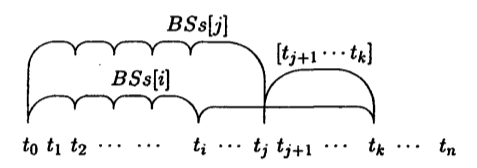
\includegraphics[width=0.5\linewidth]{viterbi_seg} \\
	\end{itemize}
\end{frame}

\begin{frame}{Approach 2: Segmentation using Branching Entropy and MDL}
	\begin{itemize}
		\item Uses the intuition that uncertainty of next character in a stream is higher at word boundaries than within words
		\item Formally, branching entropy is
			$$H(X_k|x_{k-1},..,x_{k-n}) = - \Sigma_{x \in X} P(x|x_{k-1},..,x_{k-n})log_2 P(X_k|x_{k-1},..,x_{k-n})$$
		\item Generally, we use bidirectional variant of branching entropy
		\item Uses a 3 step approach:
			\begin{itemize}
				\item Find initial segmentation by finding a good threshold for branching entropy
				\item Try possible splitting/merging of segments (local changes) in order of their costs and accept if DL decreases
				\item Try possible splitting/merging of segment types (global changes) in order of their costs and accept if DL decreases
			\end{itemize}
	\end{itemize}
\end{frame}

\begin{frame}{Evaluation}
	\begin{itemize}
		\item We compare the two approaches by measuring precision and recall of word boundary detection on the first half of the text \textit{``Alice in Wonderland''} \\
		\ \\
		\begin{table}[H]
		\centering
		\begin{tabular}{ c | c c c}\hline
		\textbf{Approach} & \textbf{Precision} & \textbf{Recall} & \textbf{F1-score} \\ \hline
		Approach 1 & 0.445 & 0.884 & 0.592 \\ 
		Approach 2 & 0.564 & 0.832 & 0.673 \\ 
		\end{tabular}
		\caption{Performance metrics of word segmentation algorithms}
		\label{tab:perf_word_seg}
		\end{table}
	\end{itemize}
\end{frame}

\begin{frame}{Approach 3: Segmentation as Search}
	\begin{itemize}
		\item Segmentation can be modeled as finding the best possible segmentation in a space of possible segmentations.
		\item AI search techniques can be used to search for these segmentations as the search space is exponential.
		\item We attempt to search for good segmentations by using Genetic Algorithms (GA).
		\item The components of the algorithm are:
		\begin{itemize}
			\item The fitness function is the negative of Description Length.
			\item An individual is represented as the indices at which the string has to be segmented.
			\item Crossover and mutation operations are defined appropriately on these individuals.
		\end{itemize} 
	\end{itemize}
\end{frame}

\section{Protein Classification}

\begin{frame}{Protein Classification}
	\begin{itemize}
		\item Classification using the segments as features is used as an extrinsic measure to evaluate the segmentations\footnote{\cite{devi2017protein}}.
		\item We use two approaches to classification:
		\begin{enumerate}
			\item Deep Learning techniques
			\item Dictionary-based segmentation followed by classification\footnote{\cite{yang2008classification}}
		\end{enumerate}
	\end{itemize}
\end{frame}
\begin{frame}{Approach 1: Classification using Deep Learning techniques}
	\begin{itemize}
		\item Proteins are sequential in nature, motivating the use of recurrent neural networks to build classification systems.
		\item The following architecture was used:
			\begin{itemize}
				\item Embed amino acids to a vector space
				\item Use an LSTM network to compute representation of protein
				\item Use a feedforward network to classify protein from the protein representation 
			\end{itemize}
		\item We obtain an average precision and average recall of 0.89 when trained over 25,000 proteins and tested over 5,000 proteins.
	\end{itemize}
\end{frame}

\begin{frame}{Approach 2: Dictionary-based Segmentation}
	The steps in dictionary-based segmentation\footnote{\cite{yang2008classification}} followed by classification are as follows:
	\begin{itemize}		
		\item Build a dictionary with maximum word length of 4 amino acids.
		\item Use a Dynamic Programming based algorithm to perform segmentation.
		\item The words of the segments of a given protein are used as features. Each protein is represented as a vector of features.
		\item An SVM with RBF kernel is trained over a train set and then tested.
		\item We obtain an average precision and average recall of 0.75 when trained over 25,000 proteins and tested over 5,000 proteins.
	\end{itemize}
\end{frame}

\begin{frame}{References}
	\bibliography{refs}
	\bibliographystyle{apalike}
\end{frame}

\end{document}


